\section{Nghiên cứu bài báo khoa học tiên tiến}

\subsection{Thông tin bài báo}

\begin{itemize}
    \item \textbf{Tên bài báo:} \textit{Generalizable Facial Expression Recognition}.
    \item \textbf{Tác giả:} Yuhang Zhang, Xiuqi Zheng, Chenyi Liang, Jiani Hu, và Weihong Deng.
    \item \textbf{Đơn vị công tác:} Beijing University of Posts and Telecommunications (BUPT).
    \item \textbf{Nơi xuất bản:} Hội nghị Châu Âu về Thị giác Máy tính (\textit{European Conference on Computer Vision - ECCV}), năm 2024. 
    \item \textbf{Xếp hạng hội nghị:} Rank A* (Hội nghị hàng đầu thế giới về Computer Vision).
    \item \textbf{Liên kết (Paper):} \url{https://eccv.ecva.net/virtual/2024/poster/718}
    \item \textbf{Mã nguồn chính thức:} \url{https://github.com/zyh-uaiaaaa/Generalizable-FER}
    \item \textbf{Từ khóa chính:} Facial Expression Recognition (FER), Zero-shot Generalization, Mask Learning, CLIP.
\end{itemize}

\subsection{Hệ thống dữ liệu thực nghiệm (Datasets)}
Trong nghiên cứu này, tác giả đã tiến hành thực nghiệm trên 05 bộ dữ liệu phổ biến nhất hiện nay trong lĩnh vực FER. Để đảm bảo tính nhất quán, tất cả dữ liệu được đưa về chuẩn 07 lớp cảm xúc cơ bản. Chi tiết các bộ dữ liệu như sau:

\begin{itemize}
    \item \textbf{RAF-DB (Real-world Affective Faces Database):}
    \begin{itemize}
        \item \textit{Đặc điểm:} Chứa 15.339 ảnh khuôn mặt từ thực tế, được gán nhãn bởi 40 chuyên gia.
        \item \textit{Phân chia:} 12.271 ảnh huấn luyện và 3.068 ảnh kiểm thử.
        \item \textit{Liên kết:} \url{https://www.kaggle.com/datasets/shuvoalok/raf-db-dataset}
    \end{itemize}

    \item \textbf{FERPlus:}
    \begin{itemize}
        \item \textit{Đặc điểm:} Là phiên bản cải tiến của FER2013 với nhãn sạch hơn và độ tin cậy cao hơn.
        \item \textit{Phân chia:} 28.709 ảnh huấn luyện và 3.589 ảnh kiểm thử.
        \item \textit{Liên kết:} \url{https://www.kaggle.com/datasets/arnabkumarroy02/ferplus}
    \end{itemize}

    \item \textbf{AffectNet:}
    \begin{itemize}
        \item \textit{Đặc điểm:} Bộ dữ liệu quy mô lớn nhất hiện nay. Trong bài báo này, tác giả tập trung vào 7 lớp cảm xúc cơ bản.
        \item \textit{Phân chia:} 286.564 ảnh huấn luyện và 4.000 ảnh kiểm thử.
        \item \textit{Liên kết:} \url{https://www.kaggle.com/datasets/mstjebashazida/affectnet}
    \end{itemize}

    \item \textbf{SFEW 2.0 (Static Facial Expressions in the Wild):}
    \begin{itemize}
        \item \textit{Đặc điểm:} Tập dữ liệu nhỏ, trích xuất từ các phân cảnh phim thực tế, có độ khó cao do điều kiện ánh sáng và góc độ.
        \item \textit{Phân chia:} 958 mẫu huấn luyện, 436 mẫu hiệu chỉnh (validation) và 372 mẫu kiểm thử.
        \item \textit{Liên kết:} \url{https://www.kaggle.com/datasets/vlntnstarodub/datasetsfew}
    \end{itemize}

    \item \textbf{MMA (Multi-Modal Affective):}
    \begin{itemize}
        \item \textit{Đặc điểm:} Bộ dữ liệu lớn thu thập từ Internet, tập trung nhiều vào người gốc Âu và Mỹ.
        \item \textit{Phân chia:} 92.968 mẫu huấn luyện, 17.356 mẫu hiệu chỉnh và 17.356 mẫu kiểm thử.
        \item \textit{Liên kết:} \url{https://www.kaggle.com/datasets/mahmoudima/mma-facial-expression}
    \end{itemize}
\end{itemize}

\subsection{Động lực nghiên cứu và ý tưởng đề xuất}

Động lực chính của nghiên cứu này xuất phát từ thực tế rằng các phương pháp tiên tiến nhất hiện nay trong lĩnh vực nhận dạng cảm xúc khuôn mặt thường suy giảm đáng kể về độ chính xác khi áp dụng trên các tập dữ liệu kiểm tra có miền khác biệt so với tập dữ liệu huấn luyện. Các mô hình hiện hành có xu hướng học quá khớp với dữ liệu nguồn, ghi nhớ cả những đặc điểm riêng của miền huấn luyện thay vì tập trung vào các đặc trưng biểu cảm mang tính phổ quát.

Vấn đề thực tiễn đặt ra là những hạn chế cố hữu của các phương pháp tổng quát hóa hoặc thích ứng miền truyền thống. Để xử lý sự khác biệt về dữ liệu, các phương pháp này thường yêu cầu hệ thống phải thu thập trước các mẫu từ miền dữ liệu đích nhằm tinh chỉnh lại mô hình. Tuy nhiên, trong triển khai thực tế, điều kiện này khó khả thi. Phân phối hoặc đặc điểm của các mẫu kiểm tra mà hệ thống gặp phải thường không thể biết trước, do đó việc tiếp cận dữ liệu mục tiêu để huấn luyện lại là bất khả thi.

Bài toán này có ý nghĩa quan trọng vì phản ánh đúng rào cản lớn nhất trong việc đưa các mô hình trí tuệ nhân tạo vào ứng dụng thực tiễn. Để hệ thống có giá trị sử dụng cao, nghiên cứu đặt mục tiêu nâng cao khả năng tổng quát hóa theo hướng zero-shot, tức là mô hình có thể hoạt động hiệu quả trên nhiều tập dữ liệu kiểm tra chưa từng thấy, với điều kiện chỉ sử dụng duy nhất một tập dữ liệu huấn luyện ban đầu. Hướng tiếp cận này được định nghĩa là bài toán nhận dạng cảm xúc khuôn mặt có khả năng tổng quát hóa.

Dựa trên bối cảnh đó, nghiên cứu được định hình nhằm tránh việc mô hình học các đặc điểm thiên lệch từ dữ liệu nguồn. Giải pháp đề xuất lấy cảm hứng từ cơ chế nhận thức tự nhiên của con người: hệ thống thị giác thường nhận diện các đặc trưng chung của khuôn mặt trước, sau đó mới tách biệt và chọn lọc các yếu tố liên quan đến biểu cảm để đánh giá. Phương pháp này tận dụng một mô hình nền tảng lớn để trích xuất đặc trưng khuôn mặt mang tính tổng quát, sau đó huấn luyện mô hình nhận dạng để tạo mặt nạ nhằm lọc ra các thông tin biểu cảm hữu ích. Cách tiếp cận này kỳ vọng sẽ giải quyết hiệu quả vấn đề tổng quát hóa, đồng thời khắc phục rào cản triển khai trong thực tiễn.

\subsection{Phát biểu bài toán và phạm vi nghiên cứu}

Nghiên cứu này tập trung vào bài toán nhận dạng cảm xúc khuôn mặt với mục tiêu nâng cao khả năng tổng quát hóa. Thay vì chỉ hướng đến việc đạt độ chính xác tối đa trên cùng một phân phối dữ liệu, phương pháp được đề xuất đặt trọng tâm vào việc cải thiện khả năng tổng quát hóa theo hướng zero-shot, tức là mô hình có thể hoạt động hiệu quả trên các tập dữ liệu kiểm tra chưa từng xuất hiện trong quá trình huấn luyện, nơi phân phối dữ liệu có sự khác biệt so với tập huấn luyện ban đầu.

Về cấu trúc dữ liệu, trong giai đoạn huấn luyện, đầu vào là một tập dữ liệu ảnh khuôn mặt duy nhất $D_{train} = \{(x_i, y_i)\}$, trong đó $x_i$ là hình ảnh khuôn mặt và $y_i$ là nhãn cảm xúc tương ứng. Về mặt kỹ thuật, hệ thống tiếp nhận các đặc trưng khuôn mặt $F$ được trích xuất và cố định trọng số từ một mô hình ngôn ngữ – hình ảnh quy mô lớn, kết hợp với đặc trưng $f$ được sinh ra từ một kiến trúc mạng học sâu khởi tạo mới, có nhiệm vụ tạo mặt nạ. Trong giai đoạn dự đoán ở môi trường thực tế, đầu vào là tập ảnh $D_{real} = \{(\tilde{x}_i, y_i)\}$ từ các miền dữ liệu đích mà hệ thống chưa từng quan sát, và hoàn toàn không có thông tin tiên nghiệm về phân phối dữ liệu.  

Đầu ra mong đợi của hệ thống là kết quả phân loại, xác định ảnh đầu vào thuộc về một trong bảy lớp cảm xúc cơ bản ($L=7$), bao gồm: ngạc nhiên, sợ hãi, ghê tởm, hạnh phúc, buồn bã, tức giận và trung tính.  

Để đảm bảo giải pháp có thể áp dụng trực tiếp trong thực tế, nghiên cứu xác lập phạm vi và ranh giới kỹ thuật cụ thể như sau:  

\begin{itemize}
    \item \textbf{Thứ nhất,} hệ thống tuyệt đối không sử dụng dữ liệu từ miền đích. Khác với các phương pháp thích ứng miền, mô hình chỉ được phép huấn luyện trên một tập dữ liệu nguồn duy nhất, không được tiếp cận bất kỳ mẫu nào từ miền dữ liệu đích để tinh chỉnh.  
    
    \item \textbf{Thứ hai,} nghiên cứu không đặt mục tiêu tối ưu hóa để đạt độ chính xác cao nhất trên miền nguồn. Trọng tâm là đánh giá khả năng tổng quát hóa đa miền. Các phương pháp trước đây thường đạt kết quả rất cao trên miền nguồn nhưng lại suy giảm mạnh khi áp dụng trên miền mới do hiện tượng ghi nhớ dữ liệu cục bộ.  
    
    \item \textbf{Thứ ba,} phạm vi phương pháp luận được giới hạn ở việc học một mặt nạ hàm sigmoid. Mô hình không học lại toàn bộ đặc trưng khuôn mặt từ đầu, mà chỉ tạo ra mặt nạ nhằm chọn lọc các thông tin liên quan đến cảm xúc từ khối đặc trưng khuôn mặt được trích xuất bởi mô hình ngôn ngữ – hình ảnh. Khi chuyển sang giai đoạn dự đoán thực tế, các khối hỗ trợ tính toán trong quá trình huấn luyện sẽ bị loại bỏ hoàn toàn, mô hình chỉ giữ lại khối phân loại để đưa ra kết quả cuối cùng.
\end{itemize}

\subsection{Giải pháp đề xuất CAFE}

\subsubsection{Ý tưởng cốt lõi}

Nghiên cứu đề xuất một phương pháp mới mang tên CAFE, được thiết kế chuyên biệt để mô phỏng cách con người nhận thức biểu cảm khuôn mặt. Khác với các phương pháp truyền thống thường huấn luyện một mạng nơ-ron từ đầu để trích xuất toàn bộ đặc trưng, dẫn đến việc mạng học luôn những thông tin đặc thù của miền dữ liệu và gây ra tình trạng học quá khớp, CAFE chia bài toán thành hai bước tiệm cận với hệ thống thị giác tự nhiên. Bước thứ nhất định vị và trích xuất các đặc trưng chung của khuôn mặt nhằm loại bỏ yếu tố khác biệt về miền dữ liệu. Bước thứ hai chỉ chọn lọc các đặc trưng liên quan mật thiết đến cảm xúc để đưa ra quyết định.

Để hiện thực hóa điều này, nguyên lý cốt lõi của CAFE là không học lại đặc trưng khuôn mặt từ đầu. Thay vào đó, kiến trúc tận dụng khả năng tổng quát hóa của một mô hình ngôn ngữ - hình ảnh lớn để lấy các đặc trưng khuôn mặt cố định, sau đó huấn luyện một mô hình chuyên biệt học cách tạo ra một mặt nạ nhằm chắt lọc thông tin hữu ích.

\subsubsection{Luồng dữ liệu qua hệ thống}

Quá trình xử lý một ảnh đầu vào $x$ được thiết kế theo luồng phân nhánh song song trước khi tiến hành hợp nhất và tính toán tối ưu hóa đa nhiệm. Cụ thể, luồng dữ liệu diễn ra như sau:

\begin{itemize}
    \item \textbf{Nhánh trích xuất khuôn mặt:} Ảnh đầu vào $x$ được đưa qua mô hình ngôn ngữ - hình ảnh lớn để trích xuất khối đặc trưng khuôn mặt tổng quát $F$. Trong nhánh này, trọng số của mạng được đóng băng hoàn toàn.
    \item \textbf{Nhánh tạo mặt nạ:} Đồng thời, ảnh $x$ đi qua mô hình nhận dạng khởi tạo mới để trích xuất đặc trưng biểu cảm thô $f$. Dữ liệu này sau đó được thay đổi kích thước và truyền qua hàm kích hoạt sigmoid để biến đổi thành ma trận mặt nạ $M_s$.
    \item \textbf{Hợp nhất dữ liệu:} Mặt nạ $M_s$ được nhân trực tiếp với đặc trưng khuôn mặt $F$ theo nguyên lý chú ý không gian, tạo ra khối đặc trưng biểu cảm đã chọn lọc $\tilde{F} = M_sF$.
    \item \textbf{Tối ưu hóa đa nhiệm:} Khối đặc trưng $\tilde{F}$ tiếp tục được sử dụng đồng thời để tính toán hàm mất mát phân loại truyền thống, đồng thời truyền qua hai khối kiến trúc mới là khối phân tách kênh và khối đa dạng kênh. Quá trình này giúp tối ưu hóa mặt nạ và đảm bảo mạng không rơi vào trạng thái học quá khớp.
\end{itemize}

Cấu trúc chi tiết về sự tương tác giữa các nhánh mạng, luồng di chuyển của các khối đặc trưng và vị trí áp dụng các hàm mất mát thành phần được minh họa cụ thể trong Hình \ref{fig:cafe_architecture} \cite{zhang2024generalizable}.

\begin{figure}[H]
    \centering
    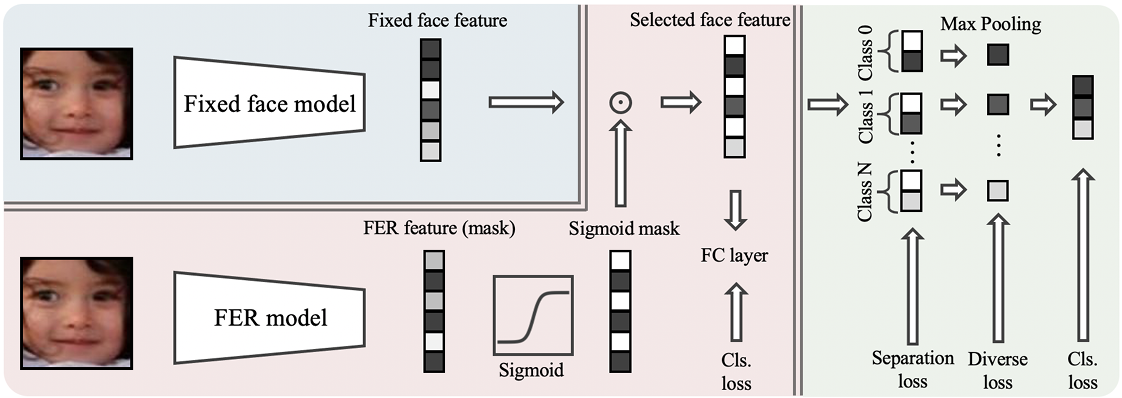
\includegraphics[width=0.9\textwidth]{images/figure2.png}
    \caption{Sơ đồ kiến trúc tổng thể của phương pháp CAFE với cơ chế học mặt nạ sigmoid và các mô-đun tối ưu hóa đa nhiệm (Trích từ Hình 2 trong \cite{zhang2024generalizable}).}
    \label{fig:cafe_architecture}
\end{figure}

\subsubsection{Kiến trúc chi tiết và các công thức cốt lõi}

\textbf{1. Khai thác đặc trưng khuôn mặt cố định}

Thay vì để mạng nhận dạng tự học đặc trưng từ đầu, nghiên cứu ứng dụng kiến trúc CLIP đã được tiền huấn luyện trên các tập dữ liệu quy mô lớn nhằm trích xuất khối đặc trưng khuôn mặt tổng quát $F$. Điểm mấu chốt của thiết kế này là toàn bộ trọng số của mô hình CLIP được đóng băng trong suốt vòng đời huấn luyện. Kỹ thuật này đóng vai trò như một màng lọc bảo vệ, ngăn chặn hệ thống vô tình nội suy và ghi nhớ các đặc trưng nhiễu từ tập dữ liệu huấn luyện cục bộ.

\textbf{2. Học mặt nạ phân bổ}

Mạng nhận dạng đảm nhiệm vai trò học cách trích xuất ma trận đặc trưng $f$, sau đó tinh chỉnh kích thước để định hình thành mặt nạ $M$. Nhằm mục đích chuẩn hóa và gia tăng tính phi tuyến, mặt nạ này được đưa qua hàm kích hoạt sigmoid:

\begin{equation}
    M_s = \text{Sigmoid}(M)
\end{equation}

Việc áp dụng hàm kích hoạt này ép các giá trị phân phối về khoảng $[0, 1]$, hoạt động tương tự như một giá trị xác suất nhằm chọn lọc các kênh đặc trưng hữu ích. Từ đó, khối đặc trưng biểu cảm cuối cùng được tính toán thông qua tích chập điểm:

\begin{equation}
    \tilde{F} = M_sF
\end{equation}

\textbf{3. Mô-đun phân tách kênh và loại bỏ lớp kết nối đầy đủ}

Trong các kiến trúc thị giác máy tính truyền thống, lớp FC thường được đặt ở tầng cuối cùng để thực hiện phân loại. Tuy nhiên, khả năng biểu diễn quá mức của lớp này dễ dẫn đến hiện tượng ghi nhớ nhãn cục bộ. Nhằm loại bỏ hoàn toàn sự phụ thuộc vào lớp FC, mô-đun phân tách tiến hành chia cắt trực tiếp khối đặc trưng $\tilde{F}$ thành bảy phần dọc theo chiều kênh, tương ứng với bảy lớp cảm xúc cơ bản.

Sau khi kết hợp với cơ chế rớt kênh ngẫu nhiên $M_{drop}$ nhằm ép mạng lan truyền sự chú ý lên toàn bộ không gian đặc trưng, hệ thống áp dụng phép toán gộp cực đại trên từng phần để trực tiếp tạo ra các giá trị xác suất phân loại dự đoán $F^d$. Quá trình tối ưu hóa khối này được thực hiện thông qua hàm mất mát phân tách $l_{sep}$ mà không cần cập nhật trọng số FC:

\begin{equation}
    l_{sep} = -\frac{1}{N} \sum_{i=1}^N \left( \log \frac{e^{F^d_{y_i}}}{\sum_{j=1}^L e^{F^d_j}} \right)
\end{equation}

\textbf{4. Hàm mất mát đa dạng kênh}

Nhằm đảm bảo bảy khối đặc trưng đại diện cho bảy biểu cảm không chứa thông tin dư thừa hoặc trùng lặp, hệ thống trích xuất ra giá trị lớn nhất dọc theo chiều kênh của mỗi phần, ký hiệu là $\tilde{F}_{max}$. Hàm mất mát đa dạng kênh $l_{div}$ được thiết kế để nới rộng các giá trị cực đại này lớn nhất có thể, từ đó ép các kênh trong mỗi phần trở nên phong phú và có ranh giới quyết định tách biệt. Phương trình hàm mất mát được định nghĩa:

\begin{equation}
    l_{div} = 1 - \frac{1}{Nc} \sum_{i=1}^N \sum_{j=1}^L \tilde{F}_{max_{ij}}
\end{equation}

\textbf{5. Tổng hàm mất mát huấn luyện}

Để hệ thống CAFE hội tụ và học được một mặt nạ tinh lọc tối ưu, tổng hàm mất mát trong quá trình huấn luyện được định nghĩa là sự kết hợp tuyến tính của cả ba thành phần chi phí:

\begin{equation}
    l_{train} = l_{cls} + \lambda l_{sep} + \beta l_{div}
\end{equation}

Trong các hệ thức toán học trên, các biến và ký hiệu được quy ước như sau:

\begin{itemize}
    \item $N$ biểu thị số lượng mẫu ảnh trong một cấu trúc dữ liệu tính toán (chẳng hạn như trong một lô nhỏ).
    \item $C$ là tổng số chiều của khối đặc trưng. Đối với cấu trúc mạng phần dư, giá trị thực nghiệm thường đạt $C = 512$.
    \item $L$ đại diện cho số lượng các lớp cảm xúc cơ bản cần phân loại, trong phạm vi nghiên cứu này $L = 7$.
    \item $y_i$ là nhãn cảm xúc thực tế của mẫu dữ liệu thứ $i$. Các chỉ số $i$ và $j$ được sử dụng để duyệt qua các chiều không gian của ma trận.
    \item Khối đặc trưng $F$, ma trận mặt nạ ban đầu $M$, và mặt nạ chuẩn hóa $M_s$ đều chia sẻ cùng kích thước không gian $N \times C$.
    \item $F^d$ là ma trận chứa các giá trị xác suất dự đoán kích thước $N \times L$. Trong đó, $F^d_{y_i}$ là giá trị tương ứng với nhãn đúng của mẫu thứ $i$, và $F^d_j$ là xác suất dự đoán cho lớp thứ $j$.
    \item $\tilde{F}_{max_{ij}}$ đại diện cho giá trị lớn nhất trích xuất được thuộc về bức ảnh thứ $i$ và lớp cảm xúc thứ $j$ trong ma trận cực đại kích thước $N \times L$.
    \item $c$ là hằng số chuẩn hóa tỷ lệ thuận với số kênh phân bổ cho mỗi lớp (thực nghiệm sử dụng $c = 73$).
    \item $\lambda$ và $\beta$ là các siêu tham số được cấu hình nhằm cân bằng mức độ đóng góp của từng khía cạnh tối ưu, với các giá trị được tinh chỉnh là $\lambda = 1.5$ và $\beta = 5$.
\end{itemize}

Trong cơ chế vận hành, $l_{cls}$ đảm bảo mặt nạ định hướng đúng đặc trưng để phân loại chính xác, $l_{sep}$ hỗ trợ gia tăng tính tổng quát thông qua việc loại bỏ tham số của lớp FC, và $l_{div}$ chịu trách nhiệm làm phong phú không gian biểu diễn biểu cảm. Khi bước vào giai đoạn suy diễn thực tế, toàn bộ các khối tính toán thuộc $l_{sep}$ và $l_{div}$ sẽ được loại bỏ khỏi biểu đồ tính toán. Luồng dữ liệu suy diễn chỉ duy trì nhánh trích xuất đặc trưng thuần túy, đảm bảo mô hình hoạt động tinh gọn và tối ưu hóa thời gian thực thi.

\subsubsection{Mục tiêu kỹ thuật và tóm lược quy trình vận hành}

Mục tiêu cốt lõi của nghiên cứu này là cải thiện khả năng tổng quát hóa zero-shot của các mô hình FER khi đối mặt với các tập dữ liệu kiểm tra hoàn toàn mới có sự khác biệt về miền dữ liệu. Cụ thể, hệ thống phải đảm bảo khả năng dự đoán chính xác trong khi chỉ được phép sử dụng duy nhất một tập dữ liệu nguồn để huấn luyện. Nghiên cứu xác lập giới hạn nghiêm ngặt là tuyệt đối không tiếp cận bất kỳ mẫu dữ liệu nào, dù có nhãn hay chưa gán nhãn, từ miền dữ liệu đích. Mục tiêu này trực tiếp giải quyết rào cản triển khai trong thực tế, nơi phân phối của các mẫu dữ liệu kiểm tra thường là biến số không thể dự báo trước.

Nhằm đạt được mục tiêu trên, phương pháp CAFE được thiết kế để mô phỏng cơ chế nhận thức biểu cảm của con người qua quy trình ba bước trọng tâm:

\begin{itemize}
    \item \textbf{Khai thác đặc trưng khuôn mặt cố định:} Hệ thống sử dụng mô hình ngôn ngữ - hình ảnh lớn như CLIP để trích xuất đặc trưng khuôn mặt tổng quát. Toàn bộ trọng số của khối đặc trưng này được đóng băng trong suốt quá trình huấn luyện.
    
    \item \textbf{Học mặt nạ sigmoid:} Mạng khởi tạo một mô hình FER mới nhằm học cách tạo ra một mặt nạ đặc trưng. Mặt nạ này được xử lý qua hàm kích hoạt sigmoid để chuẩn hóa giá trị về khoảng xác suất, sau đó nhân trực tiếp với khối đặc trưng khuôn mặt cố định để tinh lọc thông tin biểu cảm.
    
    \item \textbf{Tối ưu hóa đa nhiệm không dùng lớp FC:} Hệ thống loại bỏ hoàn toàn sự phụ thuộc vào lớp FC để giảm thiểu rủi ro học quá khớp. Khối đặc trưng sau tinh lọc được chia làm bảy phần dọc theo chiều kênh. Thông qua phép toán max pooling trên mỗi phần, mạng trực tiếp tạo ra các giá trị logit phân loại, kết hợp với hàm mất mát đa dạng kênh để tăng cường độ tách biệt giữa các biểu cảm.
\end{itemize}

\subsubsection{Phân tích cơ sở khoa học và tính hiệu quả của phương pháp}

Sự vượt trội của kiến trúc CAFE trong các thực nghiệm đa miền xuất phát từ việc thiết kế một cơ chế phòng vệ nhiều lớp, giúp hệ thống chống lại hiện tượng học quá khớp một cách bền vững. Các luận điểm chính giải thích cho hiệu quả của phương pháp bao gồm:

\textbf{Ngăn chặn sự ghi nhớ miền dữ liệu cục bộ}

Việc đóng băng trọng số của mô hình CLIP đóng vai trò như một chốt chặn kỹ thuật, đảm bảo nền tảng đặc trưng luôn duy trì được tính tổng quát hóa cao. Cơ chế này ngăn chặn hiệu quả việc mô hình FER học lây các đặc điểm nhiễu đặc thù từ tập huấn luyện như điều kiện ánh sáng, bối cảnh môi trường hoặc góc chụp ảnh. Bằng cách giữ nguyên tri thức từ mô hình lớn, hệ thống chỉ tập trung vào việc học cách khai thác thông tin thay vì thay đổi bản chất đặc trưng.

\textbf{Loại bỏ rủi ro từ lớp kết nối đầy đủ}

Trong các cấu trúc học sâu truyền thống, lớp FC sở hữu năng lực học tập và biểu diễn quá mạnh, dẫn đến xu hướng ghi nhớ nhãn của tập huấn luyện thay vì học các quy luật trừu tượng. Việc chuyển đổi bài toán nhận dạng thành dạng chia cắt kênh và gom nhóm trực tiếp đã triệt tiêu hoàn toàn khả năng học thuộc lòng của lớp mạng này. Điều này buộc mô hình phải dựa vào sự phân bổ đặc trưng trên các kênh nơ-ron để đưa ra quyết định, từ đó gia tăng độ tin cậy khi gặp các dữ liệu lạ.

\textbf{Tác dụng chuẩn hóa và tính phi tuyến của hàm sigmoid}

Hàm kích hoạt sigmoid không chỉ bổ sung tính phi tuyến cần thiết cho mô hình mà còn ép các giá trị của mặt nạ vào một khoảng chuẩn hóa. Nếu thiếu đi hàm này, hiệu suất của hệ thống sẽ suy giảm nghiêm trọng do mặt nạ mất đi tính chất xác suất trong việc chọn lọc đặc trưng. Hàm sigmoid giúp mô hình thực hiện cơ chế chú ý một cách mềm dẻo, giảm thiểu tình trạng mặt nạ bị điều chỉnh quá mức theo dữ liệu khuôn mặt đầu vào cụ thể.

\textbf{Đơn giản hóa nhiệm vụ tối ưu hóa}

Thay vì phải đảm nhận trọng trách nặng nề là học lại toàn bộ quy trình trích xuất đặc trưng biểu cảm từ con số không, việc chỉ học một mặt nạ để chọn lọc thông tin trên nền tảng tri thức có sẵn là một nhiệm vụ tối ưu hóa nhẹ nhàng và hiệu quả hơn. Thiết kế này cho phép mô hình trích xuất được các quy luật cơ bản của biểu cảm khuôn mặt mà không đòi hỏi một mạng nơ-ron có cấu trúc quá phức tạp. Hệ quả là tính bền vững của mô hình được gia tăng đáng kể, đồng thời nâng cao khả năng thích ứng chéo giữa nhiều bộ dữ liệu khác nhau trong môi trường thực tế.

\subsection{Thực nghiệm minh họa và đánh giá kết quả}

Để chứng minh tính hiệu quả của phương pháp CAFE, hệ thống thực nghiệm được thiết kế tập trung vào khả năng tổng quát hóa chéo miền. Quá trình đánh giá được thực hiện thông qua việc so sánh với các phương pháp tiên tiến nhất và phân tích chuyên sâu về sự đóng góp của từng thành phần kiến trúc.

\subsubsection{Thiết lập thực nghiệm và các phương pháp so sánh}

Nghiên cứu sử dụng năm bộ dữ liệu phổ biến bao gồm RAF-DB, FERPlus, AffectNet, SFEW2.0 và MMA. Tất cả dữ liệu đều được quy chuẩn về bảy lớp cảm xúc cơ bản. Giao thức thực nghiệm chính được áp dụng là khả năng tổng quát hóa zero-shot chéo miền. Theo giao thức này, mô hình chỉ được huấn luyện trên một miền nguồn duy nhất và tiến hành kiểm tra trực tiếp trên các miền đích còn lại mà không sử dụng bất kỳ mẫu dữ liệu nào từ miền đích để tinh chỉnh.

Hệ thống được so sánh với các phương pháp tiên tiến nhất như SCN, RUL, EAC và OFER. Ngoài ra, một phương pháp nền tảng được xây dựng bằng cách đóng băng mô hình CLIP và tinh chỉnh một lớp kết nối đầy đủ nhằm xác định xem sự cải thiện hiệu suất đến từ kiến trúc mặt nạ hay chỉ đơn thuần do sức mạnh của mô hình lớn. Nghiên cứu cũng thực hiện huấn luyện từ đầu đối với mạng xương sống để kiểm chứng tính bền vững của giải pháp.

\subsubsection{Chỉ số đo lường hiệu suất}

Trong bài toán nhận dạng cảm xúc khuôn mặt, việc lựa chọn chỉ số đo lường đóng vai trò quyết định đến tính khách quan của kết quả. Nghiên cứu sử dụng hai chỉ số chính:

\begin{itemize}
    \item \textbf{Độ chính xác tổng thể:} Phản ánh tỷ lệ phần trăm các mẫu được dự đoán đúng trên toàn bộ tập dữ liệu kiểm tra. Chỉ số này cung cấp cái nhìn khái quát về hiệu suất chung nhưng có thể gây sai lệch khi tập dữ liệu bị mất cân bằng dữ liệu.
    \item \textbf{Độ chính xác trung bình:} Đây là chỉ số quan trọng nhất, được tính bằng cách lấy trung bình cộng độ chính xác của từng lớp cảm xúc riêng biệt. Do các bộ dữ liệu thực tế thường cực kỳ mất cân bằng, chỉ số này đảm bảo mô hình không ``gian lận'' bằng cách chỉ ưu tiên nhận diện các lớp chiếm đa số mà bỏ qua các lớp thiểu số. Việc tối ưu hóa dựa trên độ chính xác trung bình phản ánh đúng năng lực tổng quát hóa và tính công bằng của hệ thống đối với mọi trạng thái cảm xúc.
\end{itemize}

\subsubsection{Kết quả thực nghiệm và phân tích chuyên sâu}

Kết quả thực nghiệm khẳng định sự vượt trội của phương pháp CAFE so với các giải pháp tiên tiến nhất trên cả năm bộ dữ liệu. Khi huấn luyện trên RAF-DB, CAFE đạt độ chính xác trung bình 63,48\% trên các tập kiểm tra chéo, vượt xa mức 54,88\% của phương pháp tốt nhất trước đó.

Nghiên cứu cắt bỏ cho thấy mọi thành phần trong kiến trúc đều đóng góp tích cực vào hiệu suất. Việc áp dụng mặt nạ giúp nâng độ chính xác trung bình từ 46,67\% lên 55,49\%. Các mô-đun phân tách và đa dạng tiếp tục cải thiện kết quả lên mức 57,17\%. Đặc biệt, nếu loại bỏ hàm kích hoạt sigmoid, hiệu suất sụt giảm nghiêm trọng xuống còn 58,05\%, chứng minh vai trò không thể thay thế của nó trong việc chuẩn hóa và chống học quá khớp.

Đáng chú ý, khi loại bỏ mạng xương sống tiền huấn luyện, CAFE vẫn duy trì được hiệu suất ổn định với mức giảm nhẹ, trong khi các phương pháp như EAC bị sụt giảm thê thảm. So sánh với phương pháp tinh chỉnh trực tiếp mô hình CLIP, CAFE cũng tạo ra khoảng cách lớn về độ chính xác. Điều này khẳng định cơ chế tạo mặt nạ mới chính là yếu tố giải phóng sức mạnh tổng quát hóa của các mô hình ngôn ngữ - hình ảnh lớn.

\subsection{Liên hệ với chương sách giáo trình nền tảng}

Mối quan hệ kỹ thuật giữa lý thuyết nền tảng trong chương sách giáo trình về nhận dạng cảm xúc khuôn mặt và bài báo hiện đại ứng dụng phương pháp CAFE thể hiện một bước tiến hóa rõ rệt của lĩnh vực. Nghiên cứu hiện đại không bác bỏ hoàn toàn hệ thống lý thuyết cũ mà trực tiếp kế thừa cấu trúc cốt lõi. Từ nền tảng đó, nghiên cứu tiến hành thay thế các công cụ phân tích thủ công bằng các cấu trúc mạng học sâu, đồng thời đưa ra lời giải trực tiếp cho những câu hỏi mở mà thế hệ đi trước để lại. Sự chuyển giao và nâng cấp kiến thức giữa hai tài liệu được phân tích chi tiết qua các khía cạnh sau.

\subsubsection{Sự kế thừa từ lý thuyết nền tảng}

\textbf{Cấu trúc ba bước tiêu chuẩn:}
Chương sách giáo trình định nghĩa một hệ thống phân tích biểu cảm khuôn mặt tự động luôn bao gồm ba giai đoạn cơ bản: thu thập khuôn mặt, trích xuất và biểu diễn dữ liệu khuôn mặt, cuối cùng là nhận dạng cảm xúc. Phương pháp đề xuất trong bài báo tuân thủ tuyệt đối triết lý cấu trúc này, nhưng hiện đại hóa từng bước thực thi thông qua việc ứng dụng công cụ tự động chuyên sâu để phát hiện khuôn mặt, sử dụng mô hình ngôn ngữ - hình ảnh để trích xuất và sử dụng cấu trúc tạo mặt nạ để phân loại.

\textbf{Hệ thống bảy lớp cảm xúc cơ bản:}
Mặc dù lý thuyết nền tảng có đề cập đến hệ thống mã hóa hành động khuôn mặt nhằm bắt giữ các chuyển động vi tế của cơ mặt, cả hai hệ thống nghiên cứu đều thống nhất sử dụng bảy biểu cảm nguyên mẫu xuất phát từ lý thuyết tâm lý học nền tảng làm mục tiêu phân loại cốt lõi. Các biểu cảm bao gồm: ngạc nhiên, sợ hãi, ghê tởm, hạnh phúc, buồn bã, tức giận và trung tính.

\textbf{Triết lý thiết kế mô phỏng nhận thức tự nhiên:}
Tài liệu giáo trình đặt ra một yêu cầu khắt khe là hệ thống máy tính phải có khả năng phân tích biểu cảm khuôn mặt bất chấp sự thay đổi của bối cảnh, giới tính hay nền văn hóa. Phương pháp CAFE đã lấy chính yêu cầu này làm kim chỉ nam thiết kế. Cụ thể, kiến trúc mô phỏng cơ chế con người định vị các đặc trưng chung của khuôn mặt để loại bỏ sự khác biệt về môi trường trước, sau đó mới tiến hành tách biệt và chọn lọc các đặc trưng biểu cảm. Khung tư duy này là tiền đề dẫn đến sự ra đời của cơ cấu mặt nạ trên nền đặc trưng cố định.

\subsubsection{Sự mở rộng và giải quyết các câu hỏi mở}

\textbf{Bài toán tổng quát hóa và thử nghiệm chéo miền:}
Các nhà nghiên cứu ở thế hệ trước đã vạch ra một giới hạn lớn của lĩnh vực khi các hệ thống thường chỉ được huấn luyện và đánh giá trên cùng một bộ dữ liệu đồng nhất, quy mô nhỏ và được kiểm soát chất lượng ánh sáng nghiêm ngặt. Do đó, khả năng tổng quát hóa của các phương pháp khi đối mặt với môi trường và bối cảnh bất định vẫn là một câu hỏi mở. Kiến trúc CAFE được sinh ra để trực tiếp giải quyết bài toán này. Hệ thống định nghĩa lại quy trình thành nhận dạng cảm xúc khuôn mặt có khả năng tổng quát hóa, trong đó cấu trúc mạng bị ép buộc phải học từ một miền dữ liệu nguồn duy nhất và kiểm chứng độ chính xác trên các tập dữ liệu kiểm tra chưa từng thấy mà không được phép tiến hành bất kỳ tinh chỉnh nào.

\textbf{Khắc phục sự khác biệt cá nhân:}
Lý thuyết nền tảng ghi nhận rằng sự khác biệt cá nhân như hình dáng, kết cấu da, sự hiện diện của râu hay kính mắt giữa các chủng tộc và độ tuổi làm suy giảm độ tin cậy của quá trình phân tích đặc trưng. Hướng tiếp cận mới giải quyết triệt để rào cản đa dạng sinh học này bằng cách sử dụng mạng xương sống đã được tiền huấn luyện trên dữ liệu web quy mô khổng lồ, đảm bảo khối đặc trưng khuôn mặt nền tảng bao quát được mọi đặc điểm nhân dạng và môi trường.

\subsubsection{Sự thay thế bởi hướng tiếp cận học sâu hiện đại}

\textbf{Thay thế phương pháp trích xuất đặc trưng:}
Trong các hệ thống kinh điển, để biểu diễn cảm xúc, quy trình phụ thuộc hoàn toàn vào nhóm đặc trưng thủ công. Nhóm này được chia làm hai loại chính: đặc trưng hình học đòi hỏi tính toán tọa độ vật lý bằng mô hình diện mạo chủ động, và đặc trưng ngoại hình sử dụng bộ lọc tần số hoặc luồng quang học để nội suy nếp nhăn. Trong kiến trúc hiện đại, toàn bộ các công cụ thủ công này bị loại bỏ. Hệ thống thay thế bằng đặc trưng học sâu thông qua mạng biến áp thị giác, tự động trích xuất một khối biểu diễn không gian đa chiều. Việc học các khoảng cách vật lý được thay thế bằng một mặt nạ sigmoid nhân trực tiếp vào khối đặc trưng nhằm tự động chắt lọc thông tin phi tuyến.

\textbf{Bước ngoặt trong kiến trúc phân loại:}
Khâu nhận dạng cảm xúc trong quá khứ thường sử dụng các bộ phân loại như máy học vector hỗ trợ hay hệ chuyên gia dựa trên luật. Nhận ra rằng các lớp kết nối đầy đủ trong mạng nơ-ron có năng lực biểu diễn quá mạnh dẫn đến hiện tượng học quá khớp cục bộ, kiến trúc hiện đại đã loại bỏ hoàn toàn tầng nơ-ron này. Giải pháp thay thế là sử dụng mô-đun phân tách kênh để chia cắt khối biểu diễn thành bảy phần, kết hợp với phép toán gộp cực đại để trực tiếp nội suy xác suất phân loại. Kỹ thuật này đã biến đổi bản chất của bài toán phân loại đa lớp truyền thống thành một dạng tương tự như cơ chế học phân phối nhãn.

\subsubsection{Phân tích đối sánh các đặc tính kỹ thuật}

Để làm rõ sự tiến hóa từ phương pháp phân tích thủ công đến việc ứng dụng sức mạnh của các mô hình học sâu lớn, Bảng \ref{tab:comparison_theory_cafe} dưới đây trình bày nội dung so sánh trực tiếp giữa hai hệ thống nghiên cứu dựa trên các khía cạnh kỹ thuật cốt lõi.

\renewcommand{\arraystretch}{1.3} % Tăng khoảng cách các dòng cho thoáng và chuyên nghiệp

\begin{longtable}{|p{0.22\textwidth}|p{0.34\textwidth}|p{0.34\textwidth}|}
    
    % --- Phần 1: Tiêu đề và Header cho trang ĐẦU TIÊN ---
    \caption{So sánh đặc tính kỹ thuật giữa hệ thống phân tích truyền thống và phương pháp CAFE hiện đại.}
    \label{tab:comparison_theory_cafe} \\
    \hline
    \textbf{Khía cạnh đối sánh} & \textbf{Lý thuyết nền tảng \newline(Phương pháp truyền thống)} & \textbf{Phương pháp CAFE \newline(Hướng tiếp cận hiện đại)} \\
    \hline
    \endfirsthead

    % --- Phần 2: Tiêu đề lặp lại ở các trang TIẾP THEO ---
    \multicolumn{3}{c}%
    {{\bfseries Bảng \thetable\ (tiếp theo)}} \\
    \hline
    \textbf{Khía cạnh đối sánh} & \textbf{Lý thuyết nền tảng \newline(Phương pháp truyền thống)} & \textbf{Phương pháp CAFE \newline(Hướng tiếp cận hiện đại)} \\
    \hline
    \endhead

    % --- Phần 3: Ghi chú ở cuối trang bị ngắt (FOOTER) ---
    \hline
    \multicolumn{3}{|r|}{\textit{Tiếp tục ở trang sau...}} \\
    \hline
    \endfoot

    % --- Phần 4: Đóng bảng ở cuối cùng (LAST FOOTER) ---
    \hline
    \endlastfoot

    % --- Phần 5: NỘI DUNG BẢNG ---
    \textbf{Mục tiêu cốt lõi} & Nhận dạng cảm xúc thông qua hệ thống AFEA gồm ba bước tiêu chuẩn, tập trung nhận diện biểu cảm trong môi trường có kiểm soát ánh sáng. & Cải thiện khả năng tổng quát hóa zero-shot trên các miền dữ liệu hoàn toàn chưa từng thấy, trực tiếp giải quyết sự khác biệt về miền dữ liệu. \\
    \hline
    \textbf{Cơ chế biểu diễn dữ liệu} & Phụ thuộc hoàn toàn vào đặc trưng thủ công, bao gồm đặc trưng hình học tính toán từ điểm mốc và đặc trưng ngoại hình tính từ kết cấu da. & Phụ thuộc vào đặc trưng học sâu, kế thừa khối đặc trưng tổng quát hóa từ mô hình ngôn ngữ - hình ảnh kết hợp với một mặt nạ tinh lọc. \\
    \hline
    \textbf{Quy trình phương pháp chính} & Thu thập khuôn mặt, định vị điểm chuẩn thủ công, trích xuất đặc trưng bằng bộ lọc và phân loại bằng học máy kinh điển (SVM, HMM). & Đóng băng trọng số đặc trưng khuôn mặt, huấn luyện mạng tạo mặt nạ sigmoid, áp dụng mô-đun phân tách kênh và hàm mất mát đa dạng kênh. \\
    \hline
    \textbf{Yêu cầu về phổ dữ liệu} & Đòi hỏi dữ liệu kiểm tra và huấn luyện có sự tương đồng phân phối. Hiệu suất giảm mạnh nếu có sự thay đổi về ánh sáng hoặc sự khác biệt cá nhân. & Chỉ sử dụng duy nhất một miền dữ liệu nguồn để huấn luyện, tuyệt đối không tiếp cận dữ liệu đích, có khả năng chạy trực tiếp chéo miền. \\
    \hline
    \textbf{Độ phức tạp tính toán} & Phức tạp chủ yếu ở khâu tiền xử lý (cắt ảnh, tính toán tọa độ đặc trưng hình học bằng AAM). Các bộ phân loại ở phần đuôi tương đối nhẹ. & Phức tạp ở quy mô của mạng trích xuất nền tảng nhưng mạng học mặt nạ cực kỳ tinh gọn do loại bỏ hoàn toàn lớp kết nối đầy đủ để chống học quá khớp. \\
    \hline
    \textbf{Khả năng ứng dụng thực tiễn} & Hoạt động ổn định trong phòng thí nghiệm, nhưng khả năng tổng quát hóa trong thế giới thực được xem là một bài toán chưa có lời giải. & Khả năng triển khai thực tế cao, phù hợp cho các hệ thống mở nơi phân phối dữ liệu và môi trường của người dùng cuối không được biết trước. \\
    \hline
    \textbf{Cơ chế xử lý nhiễu và độ lệch} & Loại bỏ độ lệch chuyển động cơ mặt bằng cách tính tỷ lệ tham số so với một ảnh khung hình có khuôn mặt trung tính hoặc căn chỉnh không gian ba chiều. & Tránh học nhiễu cục bộ bằng cách đóng băng khối đặc trưng nền tảng, đồng thời ép mạng học các quy luật biểu cảm đơn giản thông qua hàm mất mát đa dạng kênh. \\
    
\end{longtable}

Tổng hợp lại, lý thuyết trong chương sách giáo trình đóng vai trò thiết lập hệ quy chiếu vững chắc về các bước thực thi và nhận diện chính xác các rào cản ứng dụng. Dựa trên bộ khung đó, phương pháp CAFE đã thay thế toàn bộ hệ thống trích xuất đặc trưng cồng kềnh bằng các công cụ học sâu mạnh mẽ nhất. Sự dịch chuyển thế hệ này đã hiện thực hóa được mục tiêu tối thượng mà nền tảng lý thuyết từng hướng đến: xây dựng một hệ thống hoạt động bền bỉ và nhận dạng chính xác trong sự hỗn loạn của dữ liệu thế giới thực.

\subsection{Đánh giá và nhận định}

\subsubsection{Phân tích các điểm mạnh về mặt kỹ thuật}

\textbf{Thiết kế kiến trúc mô phỏng nhận thức tự nhiên:} 
Điểm mạnh cốt lõi của phương pháp nằm ở cách phân rã bài toán thành hai giai đoạn bám sát cơ chế thị giác của con người. Thay vì xử lý đồng thời, hệ thống sử dụng một mô hình ngôn ngữ - hình ảnh lớn để định vị đặc trưng khuôn mặt một cách tổng quát, sau đó sử dụng một mô hình nhận dạng chuyên biệt học cách tạo mặt nạ để chọn lọc riêng biệt các thông tin biểu cảm. Việc chuyển đổi nhiệm vụ từ học toàn bộ không gian đặc trưng sang chỉ học một mặt nạ lọc giúp giảm tải đáng kể áp lực tính toán cho mạng nơ-ron, cho phép hệ thống tập trung trích xuất các quy luật đơn giản và dễ vận dụng chéo miền hơn.

\textbf{Khả năng chống học quá khớp đa tầng:} 
Phương pháp này thiết lập một cơ chế phòng ngự chặt chẽ nhằm ngăn chặn hệ thống ghi nhớ các đặc điểm nhiễu của tập huấn luyện:
\begin{itemize}
    \item \textit{Đóng băng khối đặc trưng nền tảng:} Việc duy trì trạng thái đóng băng toàn bộ trọng số của mô hình nền tảng trong suốt chu kỳ huấn luyện giúp các khối đặc trưng khuôn mặt không bị biến dạng để chạy theo phân phối cục bộ, qua đó bảo toàn trọn vẹn năng lực tổng quát hóa nguyên bản.
    \item \textit{Tích hợp hàm kích hoạt sigmoid:} Hàm toán học này bổ sung tính phi tuyến và chuẩn hóa các giá trị của mặt nạ, biến nó thành một bộ lọc xác suất thực thụ. Dữ liệu thực nghiệm chứng minh rằng việc loại bỏ hàm này khiến hệ thống suy giảm nghiêm trọng khả năng chống học vẹt.
    \item \textit{Loại bỏ lớp kết nối đầy đủ:} Nhận thức được rủi ro ghi nhớ nhãn từ năng lực biểu diễn quá mức của lớp mạng này, kiến trúc đề xuất chia cắt khối đặc trưng thành bảy phần độc lập, sau đó ứng dụng phép toán gộp cực đại để tạo thẳng các giá trị xác suất phân loại mà không cần bất kỳ tham số kết nối dày đặc nào.
\end{itemize}

\textbf{Kỹ thuật tối ưu hóa thông minh và khả năng triển khai:} 
Song song với việc phân tách kênh, hệ thống ứng dụng hàm mất mát đa dạng kênh nhằm tối đa hóa các cực trị trong không gian biểu diễn. Kỹ thuật này ép buộc các kênh thông tin thuộc cùng một nhóm biểu cảm phải duy trì sự phong phú và tách biệt rõ rệt, giải quyết triệt để vấn đề chồng chéo ranh giới giữa các lớp cảm xúc. Nhờ đó, giải pháp thể hiện khả năng tổng quát hóa zero-shot xuất sắc, tháo gỡ hoàn toàn rào cản ứng dụng khi có thể nhận dạng chính xác trên các miền dữ liệu xa lạ chỉ với một tập huấn luyện duy nhất.

\textbf{Tính bền vững và tính độc lập với cấu trúc nền:} 
Hệ thống cho thấy độ bền vững kỹ thuật vượt trội khi không phụ thuộc vào một mạng xương sống tiền huấn luyện quá mạnh. Khi tiến hành huấn luyện từ đầu, hiệu suất chỉ suy giảm ở mức độ biên, trái ngược hoàn toàn với sự sụp đổ của các phương pháp tiên tiến khác trong cùng điều kiện. Điều này khẳng định cốt lõi sức mạnh của giải pháp đến từ chính tư duy thiết kế mặt nạ tinh lọc.

\subsubsection{Các giả định nền tảng và những giới hạn chưa được giải quyết}

Mặc dù mang lại hiệu suất khả quan, khung lý thuyết của phương pháp vẫn xoay quanh một số giả định cốt lõi và vấp phải những giới hạn nhất định trong môi trường khắc nghiệt.

\textbf{Giả định về sự kế thừa và khả năng tách biệt:} 
Nghiên cứu đặt nền móng trên giả định rằng các mô hình lớn có khả năng tổng quát hóa liền mạch không gian đặc trưng khuôn mặt cho mọi bài toán phân tích biểu cảm. Đồng thời, hệ thống tin cậy vào việc chỉ cần học được một cơ chế tạo mặt nạ tối ưu thì năng lực chuyển giao chéo miền sẽ tự động được kích hoạt và đảm bảo độ chính xác.

\textbf{Sự đánh đổi hiệu suất trên miền dữ liệu nguồn:} 
Một bài toán chưa được giải quyết trọn vẹn là làm thế nào để dung hòa giữa việc duy trì vị trí dẫn đầu trên miền dữ liệu nguồn và khả năng mở rộng sang miền dữ liệu đích. Cấu trúc hiện tại chấp nhận một sự đánh đổi hiển nhiên: nhượng bộ độ chính xác trên dữ liệu huấn luyện cục bộ để tối đa hóa điểm số trên các tập kiểm tra chưa từng thấy.

\textbf{Sự không khớp chiều không gian đặc trưng:} 
Kiến trúc bộc lộ sự thiếu linh hoạt khi phải thay đổi cấu trúc mạng. Do đặc thù tối ưu hóa cho không gian 512 chiều, việc áp dụng các mạng có năng lực biểu diễn cao hơn đòi hỏi phải sử dụng phép toán trung bình để ép chiều. Phương pháp giảm chiều thủ công này vô tình tạo ra một điểm thắt nút, giới hạn mức trần hiệu suất mà hệ thống có thể đạt tới do thiếu vắng một cơ chế chuyển đổi đặc trưng tinh vi hơn.

\textbf{Rào cản từ sự mơ hồ và dữ liệu nhiễu:} 
Thông qua phân tích ma trận nhầm lẫn, hệ thống vẫn gặp khó khăn trong việc phân ranh giới các cảm xúc mơ hồ về ngữ nghĩa, điển hình như trạng thái trung tính hoặc sợ hãi. Hơn nữa, với ràng buộc chỉ sử dụng một tập dữ liệu huấn luyện, mô hình trở nên cực kỳ nhạy cảm với dữ liệu có nhãn nhiễu hoặc chất lượng hiển thị thấp, cho thấy cơ chế lọc mặt nạ vẫn chưa đủ sức kháng cự trước sự sai lệch phân phối quá lớn ở đầu vào.

\subsubsection{Góc nhìn cá nhân về tính thực tiễn và hiệu quả}

Đánh giá một cách toàn diện, phương pháp đề xuất mang lại giá trị thực tiễn sắc bén và đại diện cho một bước chuyển mình trong phương pháp luận nghiên cứu nhận dạng cảm xúc khuôn mặt.

Về khía cạnh thực tiễn, giải pháp đã trực tiếp giải quyết rào cản lớn nhất của các phương pháp thích ứng miền truyền thống. Trong môi trường triển khai thực tế như việc cung cấp các dịch vụ API toàn cầu, việc yêu cầu thu thập trước dữ liệu người dùng để tinh chỉnh là một giả định bất khả thi về mặt kỹ thuật và quyền riêng tư. Việc hệ thống có khả năng hoạt động độc lập và ổn định trên các miền dữ liệu mù minh chứng cho độ chín muồi của thiết kế. Thêm vào đó, tính linh hoạt cao khi không kén chọn cấu trúc mạng giúp các kỹ sư dễ dàng tinh chỉnh và tích hợp vào đa dạng các hệ thống phần cứng từ biên đến đám mây.

Về phương diện hiệu quả, tư duy chấp nhận đánh đổi của phương pháp là một hướng đi khôn ngoan. Trong bối cảnh các nghiên cứu khác rơi vào vòng lặp học quá khớp cục bộ, giải pháp đã tiếp cận vấn đề từ gốc rễ. Việc mạnh dạn gỡ bỏ hoàn toàn lớp kết nối đầy đủ và khóa chặt khối đặc trưng tổng quát là những quyết định kỹ thuật quyết liệt, mang lại sự đột phá về khả năng chống học vẹt nhãn.

Dưới góc nhìn phản biện, vẫn còn đó những bài toán mở về sự phụ thuộc vào chất lượng dữ liệu mồi và điểm nghẽn trong việc đồng bộ hóa không gian biểu diễn giữa các kiến trúc mạng khác nhau. Khả năng giải mã sự mơ hồ trong các trạng thái cảm xúc chuyển tiếp cũng đòi hỏi những cải tiến sâu hơn về mặt cấu trúc chú ý. Tuy nhiên, vượt lên trên những giới hạn kỹ thuật cục bộ, đóng góp lớn nhất của nghiên cứu này là việc dịch chuyển tư duy thiết kế: kéo bài toán từ việc cố gắng chiến thắng trên các bộ tiêu chuẩn đánh giá tĩnh sang việc xây dựng một hệ thống có đủ độ bền bỉ để đối mặt với sự hỗn loạn và tính bất định của dữ liệu trong thế giới thực.

\subsubsection{Đề xuất hướng cải tiến và ứng dụng mở rộng}

Dựa trên việc phân tích các rào cản kỹ thuật của phương pháp CAFE trong quá trình thực nghiệm, nghiên cứu đề xuất một số hướng cải tiến cấu trúc và mở rộng khả năng ứng dụng thực tiễn nhằm khắc phục các giới hạn còn tồn đọng và tối ưu hóa năng lực hệ thống.

\vspace{0.5em}
\noindent\textbf{Các hướng cải tiến kỹ thuật chuyên sâu}

\begin{itemize}
    \item \textbf{Thứ nhất,} để giải quyết sự chênh lệch chiều không gian đặc trưng, thay vì sử dụng phép toán trung bình thông qua cửa sổ trượt một cách thủ công, thiết kế có thể tích hợp một khối chuyển đổi có khả năng học. Khối này, có thể được cấu trúc dựa trên mạng nơ-ron đa tầng hoặc cơ chế chú ý chéo, đóng vai trò ánh xạ các đặc trưng không gian có số chiều lớn từ mạng xương sống xuống không gian chuẩn của mô hình ngôn ngữ - hình ảnh mà không làm biến dạng các thông tin biểu cảm vi tế. Cơ chế này sẽ khai thác triệt để sức mạnh biểu diễn của các kiến trúc mạng quy mô lớn.
    
    \item \textbf{Thứ hai,} việc phân loại các trạng thái biểu cảm mơ hồ trên ảnh tĩnh luôn tiềm ẩn sai số. Hướng tiếp cận đột phá là chuyển đổi từ nhận dạng cảm xúc khuôn mặt tĩnh sang nhận dạng cảm xúc khuôn mặt động bằng cách tích hợp các bộ thích ứng thời gian như mạng GRU hoặc LSTM để lập mô hình sự thay đổi biểu cảm qua chuỗi khung hình. Song song đó, hệ thống có thể tận dụng bộ mã hóa văn bản để kết hợp các gợi ý ngôn ngữ - hình ảnh dựa trên hệ thống đơn vị hành động cơ mặt. Việc kết hợp đa phương thức này sẽ định hướng mặt nạ hội tụ chính xác hơn vào các vùng cơ mặt đặc thù, loại bỏ sự nhập nhằng ngữ nghĩa.
    
    \item \textbf{Thứ ba,} để xử lý triệt để bài toán dữ liệu huấn luyện nhiễu, kiến trúc có thể được nâng cấp bằng phương pháp học bán giám sát. Cơ chế này nhằm tận dụng các tập dữ liệu nhận dạng khuôn mặt quy mô khổng lồ chưa được gán nhãn biểu cảm. Trong quy trình này, một mạng giáo viên được huấn luyện trên tập dữ liệu có nhãn chuẩn sẽ khởi tạo các nhãn giả, từ đó hướng dẫn mạng học sinh trích xuất và tinh lọc đặc trưng từ kho dữ liệu chưa gán nhãn, giúp hệ thống tự tăng cường khả năng kháng nhiễu một cách chủ động.
    
    \item \textbf{Thứ tư,} nhằm giải quyết sự đánh đổi hiệu suất trên miền dữ liệu nguồn, một kiến trúc nhánh kép có thể được thiết lập. Một nhánh duy trì lớp kết nối đầy đủ nhằm tối ưu hóa sâu các đặc trưng cục bộ cho miền gốc, trong khi nhánh thứ hai tiếp tục duy trì cơ chế mặt nạ để bảo toàn năng lực thích ứng chéo miền. Quyết định dự đoán cuối cùng được dung hợp thông qua cơ chế học tự điều chỉnh trọng số dựa trên độ tin cậy của từng phân nhánh đối với mẫu dữ liệu đầu vào.
\end{itemize}

\vspace{0.5em}
\noindent\textbf{Tiềm năng ứng dụng thay thế trong môi trường thực tiễn}

Triết lý thiết kế mô phỏng nhận thức tự nhiên và cấu trúc tinh gọn của phương pháp không chỉ giới hạn trong môi trường học thuật mà còn đặc biệt phù hợp cho các bài toán công nghiệp phức tạp:

\begin{itemize}
    \item \textbf{Trong các hệ thống giám sát người lái xe:} Môi trường cabin thường xuyên chịu sự biến động về ánh sáng, rung lắc và góc quan sát. Việc mô hình có khả năng trích xuất đặc trưng biểu cảm độc lập với bối cảnh biến nó thành giải pháp lý tưởng để nhận diện trạng thái mệt mỏi, tức giận hay phân tâm của tài xế theo thời gian thực. Hệ thống có thể vận hành ổn định mà không đòi hỏi quá trình thu thập và huấn luyện lại dữ liệu cho từng loại camera chuyên biệt.
    
    \item \textbf{Đối với lĩnh vực tương tác người - máy:} Đặc biệt là rô-bốt hỗ trợ y tế hoặc các trợ lý ảo, yêu cầu thấu hiểu cảm xúc người dùng để đưa ra phản hồi thấu cảm là yếu tố sống còn. Khả năng tổng quát hóa zero-shot của phương pháp cho phép rô-bốt hoạt động mượt mà và tương thích tức thời khi tiếp xúc với những người dùng mới ngoài đời thực, loại bỏ hoàn toàn yêu cầu về quá trình hiệu chỉnh cá nhân hóa.
    
    \item \textbf{Công cụ phân tích độc lập đánh giá thiên lệch văn hóa:} Do các mô hình ngôn ngữ - hình ảnh lớn thường chứa đựng nội dung thiên lệch phương Tây, giải pháp này có thể được nhúng vào các mô hình hóa dựa trên tác tử để đo lường và định lượng sự bất đối xứng trong việc nhận dạng biểu cảm đa văn hóa, góp phần xây dựng các hệ thống trí tuệ nhân tạo công bằng và minh bạch hơn.
\end{itemize}